\section{Gated Recurrent Unit (GRU) Models}

\subsection{Introduction to GRU Architecture}

The Gated Recurrent Unit (GRU) is a type of recurrent neural network (RNN) designed to process sequential or time-dependent data by retaining useful temporal patterns during training. Unlike feed-forward neural networks, GRUs maintain memory across input steps, making them suitable for tasks where the past influences the future—such as financial time-series forecasting. GRUs achieve this by using gating mechanisms that determine how much historical information should be retained or forgotten during sequence processing.

GRUs contain two primary gates:

\begin{itemize}
  \item Update Gate: Controls how much of the past information should remain relevant for the next output.
  \item Reset Gate: Decides how much of the previous memory should be ignored when integrating new input signals.
\end{itemize}

This gated mechanism allows GRUs to learn long-term dependencies efficiently while avoiding vanishing or exploding gradients commonly seen in standard RNNs.

\subsection{Why GRUs Are Used in Time-Series Forecasting}

GRUs are widely used for sequential modeling due to their ability to:
\begin{itemize}
  \item Generalize well with shorter sequences and limited training samples
  \item Capture temporal relationships in noisy or irregular data
  \item Model nonlinear patterns without manually engineered lag features
\end{itemize}

In stock price forecasting, this is particularly useful because market patterns evolve gradually, yet abrupt fluctuations occur. GRUs strike a balance between memory and responsiveness, making them suitable for short-term prediction tasks such as next-day closing price forecasting.

\subsection{Advantages and Disadvantages of GRUs
Category	Details}

\begin{table}[h]
    \centering
    \begin{tabular}{|p{0.3\linewidth}|p{0.6\linewidth}|}
        \hline
        \textbf{Category} & \textbf{Details} \\
        \hline
        \hline
        \textbf{Advantages} & 
        \begin{itemize}
            \item Faster training compared to LSTM due to fewer parameters
            \item Performs well with limited data
            \item Avoids vanishing gradient problem better than simple RNNs
            \item Works effectively without feature engineering in many cases
        \end{itemize} \\
        \hline
        \textbf{Disadvantages} & 
        \begin{itemize}
            \item Slightly less expressive than LSTMs for complex long-range patterns
            \item May overfit when trained only on one stock without regularization
            \item Interpretability remains limited compared to simpler models
        \end{itemize} \\
        \hline
        \textbf{Shortcomings in Context} & 
        \begin{itemize}
            \item Requires careful hyperparameter tuning to avoid memorizing past trends
            \item Sensitivity to scaling and outlier behavior in noisy financial datasets
        \end{itemize} \\
        \hline
    \end{tabular}
    \caption{Assessment of Model Characteristics (likely GRU/Simple RNN variant)}
    \label{tab:model_assessment}
\end{table}

\subsection{Role of GRU in This Project}

GRU models were selected as a baseline and performance benchmark for stock prediction in this project. Since the dataset per individual company consists of approximately two years of daily values, the model size and structure had to balance complexity with generalization ability.

GRUs performed particularly well when trained using only raw OHLCV data. In this case, the model adapted efficiently to the stock's behavioral characteristics and produced stable and accurate predictions. However, this also made the model highly stock-specific, meaning generalization to unseen companies was limited.

When trained on broader datasets such as NIFTY50 or NIFTY200, the GRU model benefited from the additional variability but showed slight performance degradation unless tuned with regularization methods such as dropout.

\subsection{Trained GRU Model Configurations}

\subsubsection{Model 1 — GRU with Only Stock Data (No Indicators)}

This version used only the raw OHLCV features as input and trained for 60 epochs. It consisted of a single GRU layer followed by dropout and dense layers to generate the output.

\begin{table}[h]
    \centering
    \begin{tabular}{|l|c|r|}
        \hline
        \textbf{Layer (type)} & \textbf{Output Shape} & \textbf{Param \#} \\
        \hline
        \hline
        \texttt{gru (GRU)} & \texttt{(None, 64)} & 13,632 \\
        \hline
        \texttt{dropout (Dropout)} & \texttt{(None, 64)} & 0 \\
        \hline
        \texttt{dense (Dense)} & \texttt{(None, 32)} & 2,080 \\
        \hline
        \texttt{dense\_1 (Dense)} & \texttt{(None, 1)} & 33 \\
        \hline
    \end{tabular}
    \caption{Model Architecture Summary}
    \label{tab:model_summary}
\end{table}

This lightweight structure allowed fast convergence and produced strong performance for individual stock prediction, especially when dataset size was limited.

\subsubsection{Model 2 — GRU with Technical Indicators}

The second configuration incorporated engineered features, including trend, momentum, volatility, and volume-based indicators:

\begin{table}[h]
    \centering
    \begin{tabular}{|l|l|p{0.5\linewidth}|}
        \hline
        \textbf{Type} & \textbf{Indicator} & \textbf{Description} \\
        \hline
        \hline
        Trend & EMA (12, 26) & Exponential moving averages \\
        \hline
        Momentum & RSI (14) & Relative Strength Index \\
        \hline
        Volatility & ATR (14) & Average True Range \\
        \hline
        Volume-based & OBV & On-Balance Volume \\
        \hline
    \end{tabular}
    \caption{Summary of Technical Indicators}
    \label{tab:tech_indicators}
\end{table}

This version used a deeper architecture with two stacked GRU layers. It was also trained for 60 epochs.

\begin{table}[h]
    \centering
    \begin{tabular}{|l|c|r|}
        \hline
        \textbf{Layer (type)} & \textbf{Output Shape} & \textbf{Param \#} \\
        \hline
        \hline
        \texttt{gru\_1 (GRU)} & \texttt{(None, 20, 128)} & 53,760 \\
        \hline
        \texttt{dropout\_1 (Dropout)} & \texttt{(None, 20, 128)} & 0 \\
        \hline
        \texttt{gru\_2 (GRU)} & \texttt{(None, 64)} & 37,248 \\
        \hline
        \texttt{dropout\_2 (Dropout)} & \texttt{(None, 64)} & 0 \\
        \hline
        \texttt{dense\_2 (Dense)} & \texttt{(None, 32)} & 2,080 \\
        \hline
        \texttt{dense\_3 (Dense)} & \texttt{(None, 1)} & 33 \\
        \hline
    \end{tabular}
    \caption{Stacked GRU Model Architecture Summary}
    \label{tab:stacked_gru_summary}
\end{table}

Although the model improved generalization in multi-stock settings, it occasionally underperformed the non-indicator version for single-stock forecasting. This suggests that engineered indicators can introduce noise or redundancy when training data is limited.

\subsection{Summary of GRU Model Performance}

Key takeaways from the GRU experimentation include:

\begin{itemize}
  \item GRU models offer the best speed-to-accuracy balance among tested architectures.
  \item Using only raw OHLCV values yielded surprisingly strong results, especially for stock-specific forecasting.
  \item With technical indicators included, GRUs generalized better across multiple stocks but required careful tuning.
  \item GRUs represent a stable baseline model and provide a practical starting point for stock market forecasting.
\end{itemize}

\clearpage
\section{Long Short-Term Memory (LSTM) Model}

\subsection{Introduction to LSTM Architecture}

The Long Short-Term Memory (LSTM) network is an extension of recurrent neural networks designed to effectively learn patterns in sequential data while avoiding the vanishing and exploding gradient limitations present in standard RNNs. LSTMs achieve this through a gated structure consisting of input, forget, and output gates, which regulate how information flows forward through time and how much past information is retained.

The LSTM cell introduces an internal memory state (cell state) that stores useful information across longer time spans than traditional RNNs or even GRUs in some cases. This makes LSTM particularly suitable for financial time-series forecasting, where historical patterns and gradual momentum shifts can influence short-term price outcomes.

\subsection{Why LSTM Is Used for Time-Series Forecasting}

LSTM networks are widely adopted in forecasting applications because they are capable of learning temporal dependencies, handling non-linear input behavior, and capturing longer patterns in data such as trend formation and reversal sequences. In the context of stock prediction, price movement is rarely independent from its history; trends, oscillations, and volatility cycles evolve over time. LSTM models are designed to retain this form of information and are therefore an appropriate choice for next-day price forecasting.

\subsection{Advantages and Disadvantages of LSTM}

\begin{table}[h]
    \centering
    \begin{tabular}{|p{0.3\linewidth}|p{0.6\linewidth}|}
        \hline
        \textbf{Category} & \textbf{Details} \\
        \hline
        \hline
        \textbf{Advantages} & 
        \begin{itemize}
            \item Able to learn long-term dependencies more effectively than standard RNNs or GRUs
            \item Performs well on noisy sequences where patterns unfold gradually
            \item Stable training dynamics for multi-stock datasets
            \item Less prone to catastrophic forgetting
        \end{itemize} \\
        \hline
        \textbf{Disadvantages} & 
        \begin{itemize}
            \item Higher computational cost due to larger number of parameters
            \item Longer training time compared to GRU
            \item May overfit when data availability is limited unless regularization is applied
        \end{itemize} \\
        \hline
        \textbf{Project Context Limitations} & 
        \begin{itemize}
            \item When trained on a single stock, LSTM models may learn stock-specific behavior too well, reducing cross-stock generalization
            \item Performance benefit compared to GRU is noticeable mainly when the dataset size increases
        \end{itemize} \\
        \hline
    \end{tabular}
    \caption{Assessment of LSTM Model Characteristics}
    \label{tab:lstm_assessment}
\end{table}

\subsection{Role of LSTM in This Project}

LSTM models were included to evaluate how memory-retaining architectures behave across different dataset scales and feature complexity. The LSTM models trained in this project showed strong results both in single-company and multi-company scenarios.

When trained on only OHLCV data, the LSTM model demonstrated smooth prediction behavior and closely followed price movements. Similar to the GRU model, this setup performed exceptionally well for stock-specific forecasting, although this accuracy partially stems from the model's capacity to memorize the stock's internal movement pattern.

When trained using additional technical indicators and broader datasets such as NIFTY50 and NIFTY200, the LSTM architecture generalized better than GRU, particularly in diverse market conditions. This suggests that the LSTM structure is better suited for representing multi-phase temporal patterns that occur across companies and industries.

\subsection{Trained LSTM Model Configurations}

\subsubsection{LSTM Model Without Indicators}

The first LSTM configuration used only raw OHLCV inputs. The model consisted of two stacked LSTM layers followed by dropout and dense layers. It was trained for 60 epochs and performed strongly in single-stock forecasting, showing stable behavior during training and smooth response curves.

Model Summary: LSTM Without Indicators

\begin{table}[h]
    \centering
    \begin{tabular}{|l|c|r|}
        \hline
        \textbf{Layer (type)} & \textbf{Output Shape} & \textbf{Param \#} \\
        \hline
        \hline
        \texttt{lstm (LSTM)} & \texttt{(None, 20, 128)} & 68,608 \\
        \hline
        \texttt{dropout (Dropout)} & \texttt{(None, 20, 128)} & 0 \\
        \hline
        \texttt{lstm\_1 (LSTM)} & \texttt{(None, 64)} & 49,408 \\
        \hline
        \texttt{dropout\_1 (Dropout)} & \texttt{(None, 64)} & 0 \\
        \hline
        \texttt{dense (Dense)} & \texttt{(None, 32)} & 2,080 \\
        \hline
        \texttt{dense\_1 (Dense)} & \texttt{(None, 1)} & 33 \\
        \hline
    \end{tabular}
    \caption{Stacked LSTM Model Architecture Summary}
    \label{tab:stacked_lstm_summary}
\end{table}

\subsubsection{LSTM Model With Indicators}

A second variation was trained using additional engineered features, aligning with the indicator set used in the GRU experiments. This configuration improved the model's ability to generalize across multiple stocks, particularly within NIFTY index datasets.

\begin{table}[h]
    \centering
    \begin{tabular}{|l|c|c|}
        \hline
        \textbf{Feature} & \textbf{GRU Model} & \textbf{LSTM Model} \\
        \hline
        \hline
        Architecture & \texttt{128$\rightarrow$64 GRU} & \texttt{128$\rightarrow$64 LSTM} \\
        \hline
        Parameters & Fewer & Slightly more \\
        \hline
        Long-term memory & Moderate & \textbf{Stronger} \\
        \hline
        Training speed & \textbf{Faster} & Slower \\
        \hline
        Use case & Noisy short-term data & Trendy long-term sequences \\
        \hline
    \end{tabular}
    \caption{Comparison of GRU vs. LSTM Architectures}
    \label{tab:gru_lstm_comparison}
\end{table}

Model Summary: LSTM With Indicators

\begin{table}[h]
    \centering
    \begin{tabular}{|l|c|r|}
        \hline
        \textbf{Layer (type)} & \textbf{Output Shape} & \textbf{Param \#} \\
        \hline
        \hline
        \texttt{lstm (LSTM)} & \texttt{(None, 20, 128)} & 71,168 \\
        \hline
        \texttt{dropout\_3 (Dropout)} & \texttt{(None, 20, 128)} & 0 \\
        \hline
        \texttt{lstm\_1 (LSTM)} & \texttt{(None, 64)} & 49,408 \\
        \hline
        \texttt{dropout\_4 (Dropout)} & \texttt{(None, 64)} & 0 \\
        \hline
        \texttt{dense\_4 (Dense)} & \texttt{(None, 32)} & 2,080 \\
        \hline
        \texttt{dense\_5 (Dense)} & \texttt{(None, 1)} & 33 \\
        \hline
    \end{tabular}
    \caption{Stacked LSTM Model Architecture Summary}
    \label{tab:lstm_architecture_3}
\end{table}

A comparative observation between the two configurations showed that:

\begin{itemize}
  \item The indicator-based LSTM model generalized better when trained on multiple companies.
  \item The non-indicator model remained highly effective for a single company, especially when trained on two-year datasets.
  \item This reinforces the idea that feature engineering provides benefit primarily when dataset diversity increases.
\end{itemize}

\subsection{Performance Summary}

The evaluation results demonstrated that the LSTM architecture provided a consistent balance between accuracy, generalization, and robustness. While GRU models trained faster and often matched performance on single-company prediction tasks, LSTM models achieved stronger results when scaling to larger datasets and incorporating additional features.

Overall, LSTM forms a key component of the modelling framework explored in this project and serves as a high-performing baseline against which more complex architectures such as CNN-LSTM and Transformer models were assessed.

\clearpage

\section{Transformer Model}

\subsection{Introduction to the Transformer Architecture}

The Transformer architecture was originally introduced for sequence-to-sequence learning tasks in natural language processing, where capturing complex contextual relationships and long-range dependencies is essential. Unlike traditional recurrent neural network architectures, Transformers do not rely on sequential processing. Instead, they use self-attention mechanisms that allow the model to evaluate the importance of different time steps relative to one another within the input sequence.

This mechanism enables the network to weigh which portions of the historical sequence are most relevant to the prediction task at any given time. Because attention is computed in parallel rather than iteratively, Transformers are computationally efficient at scale and capable of modeling longer temporal patterns than recurrent models without degradation in memory retention.

\subsection{Motivation for Using Transformers in Time-Series Forecasting}

Transformers have recently gained adoption in financial forecasting because of their ability to:

\begin{itemize}
  \item Capture long-term dependencies without recursive backpropagation
  \item Process sequences in parallel, improving learning efficiency
  \item Adapt dynamically to context, allowing the model to automatically prioritize relevant historical points
\end{itemize}

Stock movement patterns often depend on trends that evolve gradually, followed by sudden shifts triggered by market sentiment or volatility changes. The attention mechanism provides an analytical advantage because it allows the model to focus on these critical points rather than uniformly weighting past observations.

\subsection{Advantages and Disadvantages of Transformers}

\begin{table}[h]
\centering
\caption{Analysis of a Deep Learning Model (Likely Transformer/Self-Attention-based) for Time Series Prediction}
\label{tab:model_analysis}
\begin{tabular}{|p{0.3\textwidth}|p{0.6\textwidth}|}
\hline
\textbf{Category} & \textbf{Observations} \\
\hline
\multirow{4}{*}{\textbf{Advantages}} & $\bullet$ Able to learn long-range and non-linear dependencies \\
& $\bullet$ Scales efficiently to large datasets \\
& $\bullet$ Attention mechanism helps prioritize meaningful time steps \\
& $\bullet$ Performs well when incorporating multiple feature types \\
\hline
\multirow{3}{*}{\textbf{Disadvantages}} & $\bullet$ Requires substantially more data to train effectively \\
& $\bullet$ More computationally demanding during both training and tuning \\
& $\bullet$ Prone to underfitting on small datasets due to model complexity \\
\hline
\multirow{4}{*}{\textbf{Contextual Limitations in This Project}} & $\bullet$ Underperformed when trained only on NIFTY50 or NIFTY200 datasets \\
& $\bullet$ Required full multi-stock data to achieve stable prediction patterns \\
& $\bullet$ Less effective compared to LSTM when only OHLCV inputs were available \\
\hline
\end{tabular}
\end{table}

\subsection{Role of Transformers in This Project}

Transformers were included to examine how modern attention-based architectures perform relative to RNN-based approaches in forecasting next-day closing prices. The evaluation focused on determining whether the architecture could uncover higher-level temporal structure across multiple stocks in the Indian market, especially when technical indicators were included.

The experiments demonstrated that Transformers required significantly more data than recurrent architectures to obtain meaningful predictions. When trained using only raw OHLCV data or limited index-based datasets, the model typically underfit and produced weaker forecasting results. However, when trained on the full dataset containing multiple NSE-listed companies and additional features, the performance improved and moved closer to the accuracy produced by tuned LSTM models.

\subsection{Trained Transformer Model Configurations
Transformer Model Without Indicators}

The first configuration used raw OHLCV features with a sequence length of 20 time steps. The model consisted of two stacked transformer encoder layers followed by a global pooling layer and fully connected output network. It was trained for 60 epochs using a batch size of 16.

\begin{table}[h]
\centering
\caption{Model Architecture Summary}
\label{tab:model_summary}
\begin{tabular}{|l|c|r|}
\hline
\textbf{Layer (type)} & \textbf{Output Shape} & \textbf{Param \#} \\
\hline
input\_layer\_1 (InputLayer) & (None, 20, 5) & 0 \\
\hline
add (Add) & (None, 20, 5) & 0 \\
\hline
transformer\_encoder (TransformerEncoder) & (None, 20, 5) & 1,194 \\
\hline
transformer\_encoder\_1 (TransformerEncoder) & (None, 20, 5) & 1,194 \\
\hline
global\_average\_pooling1d (GlobalAveragePooling1D) & (None, 5) & 0 \\
\hline
dropout\_8 (Dropout) & (None, 5) & 0 \\
\hline
dense\_6 (Dense) & (None, 64) & 384 \\
\hline
dropout\_9 (Dropout) & (None, 64) & 0 \\
\hline
dense\_7 (Dense) & (None, 1) & 65 \\
\hline
\end{tabular}
\end{table}

Transformer Model With Indicators

A second configuration incorporated the same set of engineered features used in previous GRU and LSTM experiments. This increased the model’s input dimensionality and provided more structural information to the attention mechanism.

The model architecture remained similar, with stacked encoder blocks and dropout regularization, but required more parameters due to the increased feature size. It was also trained for 60 epochs using a batch size of 16.

\begin{table}[h]
\centering
\caption{Model Architecture Summary}
\label{tab:model_summary_2}
\begin{tabular}{|l|c|r|}
\hline
\textbf{Layer (type)} & \textbf{Output Shape} & \textbf{Param \#} \\
\hline
input\_layer\_4 (InputLayer) & (None, 20, 10) & 0 \\
\hline
add\_1 (Add) & (None, 20, 10) & 0 \\
\hline
transformer\_encoder\_1 (TransformerEncoder) & (None, 20, 10) & 3,124 \\
\hline
transformer\_encoder\_2 (TransformerEncoder) & (None, 20, 10) & 3,124 \\
\hline
global\_average\_pooling1d (GlobalAveragePooling1D) & (None, 10) & 0 \\
\hline
dropout\_13 (Dropout) & (None, 10) & 0 \\
\hline
dense\_12 (Dense) & (None, 64) & 704 \\
\hline
dropout\_14 (Dropout) & (None, 64) & 0 \\
\hline
dense\_13 (Dense) & (None, 1) & 65 \\
\hline
\end{tabular}
\end{table}

\subsection{Performance Summary}

\begin{table}[h]
\centering
\caption{Comparison of Recurrent Neural Network (RNN) Architectures}
\label{tab:rnn_comparison}
\begin{tabular}{|l|p{3.5cm}|p{3.5cm}|p{3.5cm}|}
\hline
\textbf{Model} & \textbf{Strength} & \textbf{Weakness} & \textbf{When to Use} \\
\hline
GRU & Light \& fast & May miss long-term patterns & Quick prototypes \\
\hline
LSTM & Strong memory (handles vanishing gradient) & Slightly slower, more complex architecture & Stable trends \\
\hline
Transformer & Handles long-range relations, scalable, parallelizable & Heavier, needs more data & Advanced / larger datasets \\
\hline
\end{tabular}
\end{table}

The performance evaluation showed that Transformers demonstrated potential when data volume and feature diversity increased. While the architecture did not outperform the LSTM model in this project, the experiments confirmed the following trends:

\begin{itemize}
  \item Transformers benefit substantially from broader training examples across multiple companies.
  \item Technical indicators improved stability and error consistency compared to using raw values alone.
  \item The architecture performed best on the largest dataset tested but remained close in accuracy to LSTM rather than exceeding it.
\end{itemize}

These outcomes suggest that the Transformer architecture is viable for stock forecasting when sufficient data is available and can serve as a strong model candidate as future iterations incorporate sentiment analysis, intraday signals, or larger multi-stock sequencing.

\clearpage

\section{Conv1D + LSTM Hybrid Model}

\subsection{Introduction to the Hybrid Architecture}

The Conv1D + LSTM hybrid model combines the strengths of convolutional neural networks (CNNs) and recurrent architectures to model temporal structure in financial time-series data. The 1-Dimensional Convolutional layers act as feature extractors that identify local temporal patterns, such as small waveforms, trend shifts, or repeating microstructures found in price movements. These extracted temporal feature maps are then passed to an LSTM layer, which processes them sequentially to learn longer-term dependencies and temporal relationships.

This layered design allows the model to benefit from both local pattern detection offered by CNNs and sequence-level learning achieved through recurrent memory. The architecture is well-suited for forecasting scenarios where short-term fluctuations accumulate into broader directional trends, a behavior frequently observed in equity price movement.

\subsection{Motivation for Using a Hybrid Model in Time-Series Forecasting}

Pure sequential models such as LSTM or GRU tend to treat all time steps equally, which may dilute key short-term patterns—especially in financial data where recent movements and volatility surges may carry higher predictive weight. By contrast, convolutional layers selectively amplify short-term structures before passing them into the recurrent model.

This hybrid design helps address:
\begin{itemize}
  \item Rapid fluctuation capture
  \item Local trend compression
  \item Feature smoothing before sequence modeling
\end{itemize}

As a result, Conv1D + LSTM models can learn meaningful representations from noisy datasets, which aligns well with the nature of stock market signals.

\subsection{Advantages and Disadvantages of the Hybrid Model}

\begin{table}[h]
\centering
\caption{Analysis of a Hybrid Deep Learning Model (Likely CNN-LSTM)}
\label{tab:hybrid_model_analysis}
\begin{tabular}{|p{0.3\textwidth}|p{0.6\textwidth}|}
\hline
\textbf{Category} & \textbf{Observations} \\
\hline
\multirow{4}{*}{\textbf{Advantages}} & $\bullet$ Captures both short-range (CNN) and long-range (LSTM) dependencies \\
& $\bullet$ More resilient to noise than LSTM-only models \\
& $\bullet$ Can extract meaningful patterns even with moderate feature engineering \\
& $\bullet$ Performs well when trained on large multi-stock datasets \\
\hline
\multirow{3}{*}{\textbf{Disadvantages}} & $\bullet$ Requires more data than simple recurrent models \\
& $\bullet$ Higher computational cost and slower convergence \\
& $\bullet$ Hyperparameter tuning for convolution and LSTM layers increases complexity \\
\hline
\multirow{2}{*}{\textbf{Contextual Limitations}} & $\bullet$ Underperformed when trained on only NIFTY50/NIFTY200 datasets due to limited sequence diversity \\
& $\bullet$ Performed best when trained using the full multi-company dataset \\
\hline
\end{tabular}
\end{table}

\subsection{Role of the Hybrid Model in This Project}

The hybrid Conv1D + LSTM model was included to evaluate whether multi-stage temporal feature extraction improves forecasting performance compared to pure recurrent or attention-based architectures. The model aligned well with the goal of understanding the impact of structured feature extraction on prediction accuracy.

The experiments showed that the hybrid architecture performed better when trained using multiple companies rather than single-company data. In single-stock configurations, the Conv1D layers often extracted redundant short-term behavior that the LSTM could already capture, providing little benefit. However, when the training dataset expanded to include a diverse range of stocks, the convolutional filters identified transferable short-term market dynamics, improving generalization stability.

\subsection{Trained Configurations of the Hybrid Model}

The hybrid model followed the structure:

Input → Conv1D(64) → Conv1D(64) → LSTM(64) → Dense(32) → Dropout(0.2) → Dense(1)

\begin{figure}[h]
    \centering
    \caption{Conceptual Diagram of a CNN-LSTM Model Architecture}
    \label{fig:cnn_lstm_architecture}
    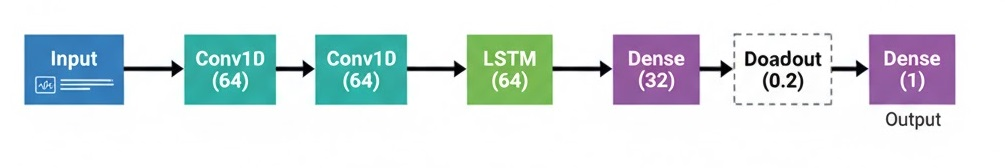
\includegraphics[width=\textwidth]{Images/methodology/cnn_lstm_model_diagram.jpg}
\end{figure}

\subsubsection{Hybrid Model Without Indicators}

The first version of the hybrid model used only OHLCV features as input. It performed well when trained on larger datasets and produced smoother and more stable predictions compared to Transformer models trained on the same data volume. The absence of indicators forced the convolutional layers to detect raw micro-patterns in the closing sequence and local relationships in open-high-low volume dynamics.

\begin{table}[h]
\centering
\caption{Model Architecture Summary}
\label{tab:cnn_lstm_summary}
\begin{tabular}{|l|c|r|}
\hline
\textbf{Layer (type)} & \textbf{Output Shape} & \textbf{Param \#} \\
\hline
input\_layer\_5 (InputLayer) & (None, 15, 5) & 0 \\
\hline
conv1d\_2 (Conv1D) & (None, 15, 64) & 1,024 \\
\hline
conv1d\_3 (Conv1D) & (None, 15, 64) & 12,352 \\
\hline
lstm\_3 (LSTM) & (None, 64) & 33,024 \\
\hline
dense\_10 (Dense) & (None, 32) & 2,080 \\
\hline
dropout\_11 (Dropout) & (None, 32) & 0 \\
\hline
dense\_11 (Dense) & (None, 1) & 33 \\
\hline
\end{tabular}
\end{table}

\subsubsection{Hybrid Model With Indicators}

A second version incorporated the engineered features used in earlier experiments. Including trend-based and volatility-based indicators expanded the dimensional richness of the input representation, providing additional structural cues for the convolutional filters. This configuration demonstrated improved generalization but required larger dataset scope to avoid overfitting.

The evaluation showed that among the tested indicator combinations, the feature set Close, MA5, and MA20 produced the most consistent results. Simpler trend-based indicators appeared to complement the convolutional layers more effectively than more volatile constructs such as ATR or RSI.

\begin{table}[h]
\centering
\caption{Model Architecture Summary (Likely CNN-LSTM)}
\label{tab:cnn_lstm_summary_2}
\begin{tabular}{|l|c|r|}
\hline
\textbf{Layer (type)} & \textbf{Output Shape} & \textbf{Param \#} \\
\hline
input\_layer\_7 (InputLayer) & (None, 15, 10) & 0 \\
\hline
conv1d (Conv1D) & (None, 15, 64) & 1,984 \\
\hline
conv1d\_1 (Conv1D) & (None, 15, 64) & 12,352 \\
\hline
lstm\_2 (LSTM) & (None, 64) & 33,024 \\
\hline
dense\_14 (Dense) & (None, 32) & 2,080 \\
\hline
dropout\_15 (Dropout) & (None, 32) & 0 \\
\hline
dense\_15 (Dense) & (None, 1) & 33 \\
\hline
\end{tabular}
\end{table}

\subsection{Performance Summary}

The Conv1D + LSTM hybrid model showed strong potential as a forecasting framework when sufficient training data was available. While the architecture did not surpass the LSTM model in single-stock configurations, it performed competitively when trained using large, multi-stock datasets and selected indicators. The results demonstrate that hybrid models can provide value in forecasting settings where both short-term fluctuations and broader momentum behaviors must be combined into a unified predictive structure.